\documentclass[paper=a4,notitlepage,parskip=half,plainheadsepline]{scrartcl}

\usepackage{silence}
\WarningsOff[everypage]% Suppress warnings related to package everypage
\usepackage{snapshot} 
\usepackage{scrlayer-scrpage} 
\usepackage{iftex}
\usepackage[ngerman]{babel}
\usepackage{graphicx}
\usepackage{float}
\usepackage[T1]{fontenc}
\usepackage[utf8]{inputenc}
\usepackage{pifont}
\usepackage{amsmath}
\usepackage[german]{varioref}
\usepackage[text={6.8in,9.6in},top=0.7in,centering]{geometry}
\usepackage{datetime2}
\usepackage{array,multirow,tabularx}
\usepackage{listingsutf8}
\usepackage[table,svgnames,dvipsnames]{xcolor}
\usepackage[most,breakable,skins,listingsutf8]{tcolorbox}
%\tcbuselibrary{listingsutf8}
\usepackage[color=blue!90,scale=0.8,placement=bottom,vshift=1.2cm]{background}
\usepackage{array}
\usepackage{physics}
\usepackage{tikz}
\usepackage{pgfplots}
\usepgflibrary{shapes.symbols}
\usetikzlibrary{arrows}
\pgfplotsset{compat=1.16}

%%%%%%%%%%%%%%%%%%%%%%%%%%%%%%%%%%%%%%%%%%          Aufgabe oder Loesung 
\newif\ifloesung
\loesungtrue
%\loesungfalse
%%%%%%%%%%%%%%%%%%%%%%%%%%%%%%%%%%%%%%%%%%%%%%%%%%%%%%%%%%%%%%%%%%%%%%%%%

%\backgroundsetup{contents={Version vom \today}}
\backgroundsetup{contents={Version vom \today}}
%\pagestyle{empty}

\pagestyle{scrheadings}
\clearpairofpagestyles
\ihead{Fachinformatiker Anwendungsentwickler~/~Informatik--Studenten}
\chead{}
\ohead{C/Python--Programmierung}
\ifoot{Frank Zimmermann}
\cfoot{SVLFG}
\ofoot{}
\ofoot{\pagemark}

\graphicspath{{./jpg/}}
\DeclareGraphicsExtensions{.jpg,.eps,.png}
%\usepackage{courier}


%\newcommand\bashprompt{\textcolor{cyan}{\small\ttfamily\bfseries{bob@remotehost{\textcolor{black}:}\textcolor{cyan!60}{\url{~}}{\textcolor{black}\$ }}}}
\newcommand\bashprompt{\textcolor{red!25!white}{\small\ttfamily\bfseries bash\$> }}
\newcommand\noprompt{\hspace{0.6cm}}
\newcommand{\startBash}{\gdef\myprompt{\bashprompt}}
\newcommand{\startNone}{\gdef\myprompt{\noprompt}}

\newcommand{\mingw}{\textsl{MinGW}}
\newcommand{\bash}{\emph{bash}}
\newcommand{\msys}{\textsl{MSYS}}
\newcommand{\git}{\emph{Git}}
\newcommand{\gcc}{\emph{gcc}}
\newcommand{\listingsfont}{\ttfamily}
\newcommand{\sh}{\texttt{pirate.c}}
\newcommand{\s}{\texttt{pirate}}

\RedeclareSectionCommand[
  beforeskip=-1\baselineskip,
  afterskip=.5\baselineskip]{section}
\RedeclareSectionCommand[
  beforeskip=-.75\baselineskip,
  afterskip=.5\baselineskip]{subsection}
\RedeclareSectionCommand[
  beforeskip=-.5\baselineskip,
  afterskip=.25\baselineskip]{subsubsection}
\RedeclareSectionCommand[
  beforeskip=.5\baselineskip,
  afterskip=-1em]{paragraph}
\RedeclareSectionCommand[
  beforeskip=-.5\baselineskip,
  afterskip=-1em]{subparagraph}

% Wenn pdflatex benutzt wird sollen die 
% installierten! frutiger-Fonts verwendet werden
% Ansonsten die TeX-eigenen cmbright
\ifPDFTeX %
\usepackage[scaled=0.90]{frutiger}
\renewcommand\familydefault{\sfdefault}
%\DeclareFixedFont\ott{T1}{phv}{mc}{n}{10pt
\else
\usepackage{cmbright}
\fi

\newfont{\lf}{svlfg scaled 2000}%
\newcolumntype{P}[1]{>{\centering\arraybackslash}p{#1}}

\ifloesung
\newtcbinputlisting[auto counter,list inside=lol,list type={lstlisting}]{\mylisting}[4][]{%
  toptitle=2mm,
  bottomtitle=2mm,listing only,
  colback=lightgray,
  %colback=yellow!10,
  listing file={#3},
  listing options={language=#4,
  aboveskip=5pt,
  belowskip=5pt,
  columns=flexible,
  keywordstyle=\color{blue},
  basicstyle=\footnotesize\listingsfont},
  colback=white,
  %colframe=gray!75!black,
  colframe=yellow!50!black,
  listing only,
  fonttitle=\bfseries,
  breakable,
  %title={Soubor \thetcbcounter: #2},
  title=Musterlösung für \texttt{#3},
  #1
}
\fi

\begin{document}
\tcbset{enhanced,colback=green!5!white, boxrule=0.5pt, colframe=green!35!black,fonttitle=\bfseries\Large}
        % \begin{tcolorbox}[drop lifted shadow]
        % This is a tcolorbox.
        % \end{tcolorbox}\par\bigskip
        \begin{tcolorbox}[toptitle=3mm,bottomtitle=3mm,title=\centering{{\lf J}\hfil Ausbildung Fachinformatiker Anwendungsentwicklung\hfil {\lf J}},
          drop lifted shadow=gray]
        \centering{\vspace{0.5cm}\LARGE Programmierübung %
        \ifloesung (mit Musterlösung)\fi}\\[0.3cm]
        \centering{C/Python--Programmierung / Simulation}\\\vspace{0.5cm}
        \end{tcolorbox}

\section{Aufgabe}
Es ist ein Programm (\texttt{pirate.exe} bzw. \texttt{pirate.py}) in der Programmiersprache C und der Programmiersprache \texttt{Python} zu schreiben, das folgendes Szenario lösen kann:

Ein Handelsschiff segelt mit konstanter Geschwindigkeit ($v_h$) in einem kartesischen Koordinatensystem vertikal in y--Richtung. Es befindet sich anfänglich an der Position $(x_0,0)$ und sein Weg kann beschrieben werden durch die Kurve $x(t) = x_0$ und $y(t) = v_h t$.

Ein Piratenschiff an den Koordinaten $(0,0)$ segelt zeitgleich mit dem Handelsschiff los und nimmt permanent Kurs auf die aktuelle Position des Handelsschiffs. Natürlich ist das Piratenschiff schneller, es hat die Geschwindigkeit $v >v_h$. D.h. $n = \frac{v_h}{v} < 1$. Wählt man also geeignete Einheiten, so kann man für die Berechnung setzen:
$x_0=x_h=1$,$v = 1$ und $v_h = n < 1$ (Konkret zu Berechnung: $n=3/4$).

Irgendwann wird das Piratenschiff das Handelsschiff eingeholt haben. Die Frage ist:

An welcher y--Position $y_{h0}$ hat das Piratenschiff das Handelsschiff eingeholt.
Da das Handelsschiff mit konstanter Geschwindigkeit segelt, ist die Frage natürlich äquivalent zu der Frage, zu welcher Zeit $t_{h0} = \frac{y_{h0}}{v_{h}}$.

\pgfplotsset{every tick label/.append style={font=\tiny}}
  
\newcommand{\cn}{0.75}
\newcommand{\yf}{12/7}
\begin{center}
\begin{tikzpicture}[scale=1.6]
\begin{axis}[
clip mode=individual,
  axis lines=middle,
  samples=200,
  grid=both,
    grid style={line width=.1pt, draw=gray!10},
%    major grid style={line width=.1pt,draw=gray!10},
%    minor grid style={line width=.1pt,draw=gray!10},
%        minor x grid style={dotted,black,thin},
%        minor y grid style={dotted,black,thin},
    ymin=0,
    ymax=2.0,
    xmin=0,
    xmax=1.25,
%    axis on top=true,
    axis x line=middle,
    axis y line=middle,
    minor x tick num = 4,
    minor y tick num = 4,
  xtick={0.0,0.5,1.0},
  ytick={0.0,1.0,...,2.0},
]
%\addplot[blue,thick,domain=0.0:1] { 0.75 / (1-(0.75)^2)+ 0.5 * (1-x) * ( ((1-x)^(0.75) / (1+0.75)) - ((1-x)^-(0.75) / (1-0.75)))};
\addplot[blue, ultra thick,domain=0.0:0.75] { \cn / (1-\cn^2) + 0.5 * (1-x) * ( (1-x)^\cn/(1+\cn) - (1-x)^(-\cn) / (1-\cn))};
\addplot[blue,ultra thick,domain=0.75:1.0,dashed] { \cn / (1-\cn^2) + 0.5 * (1-x) * ( (1-x)^\cn/(1+\cn) - (1-x)^(-\cn) / (1-\cn))};
%\draw[step=2.0](axis cs:0,0) grid(axis cs:1,2);
\node [anchor=north] at (axis cs:0,0) {$\scriptstyle O$};
\draw[red!70,thick,dotted] (axis cs:0,\yf) -- (axis cs:1,\yf);
\draw[red!70,thick,dotted] (axis cs:1,0) -- (axis cs:1,\yf);
\draw (axis cs:1,\yf) node[starburst, fill=yellow, draw=red, line width=1pt,scale=0.5] {Attack};
\draw (axis cs:1.04,0.06) node{$\scriptstyle x_0$};

\draw[semithick,gray] (axis cs:0.75,0.325) -- (axis cs:1.2,0.325);
\draw[semithick,gray] (axis cs:1,0.65) -- (axis cs:1.2,0.65);

\draw[semithick,gray] (axis cs:0.75,0.325) -- (axis cs:0.75,0.0);
\draw[semithick,gray] (axis cs:1,0.325) -- (axis cs:1.0,0.0);

\draw[semithick,black] (axis cs:0.75,0.325) -- (axis cs:1.0,0.65);

\draw (axis cs:0.66,0.43) node{$\scriptstyle(x,y)$};
% \filldraw (axis cs:0.75,0.325) circle (0.02);
% \filldraw (axis cs:1,0.65) circle (0.02);

\draw (axis cs:1.15,0.44) node{$\scriptstyle v_h t - y$};
\draw[densely dashed,latex-latex] (axis cs:1.05,0.65) -- (axis cs:1.05,0.325);
\draw (axis cs:0.89,0.17) node{$\scriptstyle x_0 -x$};
\draw[densely dashed,latex-latex] (axis cs:0.75,0.24) -- (axis cs:1.0,0.24);

\draw (axis cs:0.85,0.325) arc [start angle=0, end angle=34, x radius=0.1,y radius=0.2];
\draw (axis cs:0.88,0.41) node{$\scriptstyle \phi$};
\draw (axis cs:-0.05,\yf) node{$\scriptstyle y_{h0}$};

\node [draw, circle, fill=teal, minimum size=6.5,inner sep=0.05] at (0.75,0.325) {};
\node [draw, circle, fill=teal, minimum size=6.5,inner sep=0.05] at (1,0.65) {};
\end{axis}
\end{tikzpicture}
\end{center}


\section{Vorgehensweise}
Simulieren Sie in kleinen Zeitschritten $\Delta t$ die Bewegung beider Schiffe.
Sie bekommen durch Wahl des geeigneten Zeitschritts ein hinreichend genaues Ergebnis.

% \begin{itemize}
% \item[$t=0:$] $P_p = (0,0)$, $P_h = (1,0)$
% \item[$t=\Delta t:$] $P_p = (?,?)$, $P_h = (1,n*\Delta t)$
% \item[$t=2\Delta t:$] $P_p = (?,?)$, $P_h = (1,n*2\Delta t)$
% \item[$t=\dots$] \ldots
% \end{itemize}

Die beiden Schiffe treffen aufeinander, wenn der Abstand beider Schiffe sowohl in $x$--Richtung als auch in $y$--Richtung kleiner als $\epsilon$ ist. Dabei ist $\epsilon$ geeignet zu wählen. Die Wahl von $\epsilon$ und $\Delta t$ sind voneinander abhängig, denken Sie darüber nach.

Zur Erleichterung wurde schon die notwendige Tabelle erstellt. Diese ist folgendermaßen von links nach rechts und oben nach unten zu lesen.

\begin{enumerate}
\item[1.] Für ein bestimmtes $t$ (also auch $k$) werden die Position für das Handelsschiff $P_h=(x_h, y_h)$ und die Positionen des Piratenschiffes $P=(x, y)$ berechnet.
\item[2.] Es wird der (Kurs--)Winkel zwischen dem Handelsschiff und dem Piratenschiff aus den Abständen mit Hilfe des $\arctan()$ berechnet.
\item[3.] Mit dem Kurswinkel kann nun das jeweilige $\Delta x$ und $\Delta y$ berechnet werden, die das Piratenschiff im nächsten Zeitintervall vorwärts segelt.
\end{enumerate}
\renewcommand{\arraystretch}{1.8}
\begin{tabular}{|c|c|c|c|c|c|c|c|c|}
\hline
\rowcolor{lightgray}
$k$ & $t$           & $x_h$ & $y_h$         & $x$                           & $y$                               & $\tan \phi$ & $\Delta x$ & $\Delta y$ \\
\hline
$0$ & $0$         & 1     &$0$ &$0$       & $0$                             &$0$& $\Delta t$          & $0$ \\
\hline 
$1$ & $1\Delta t$ & 1     &$1n\Delta t$   &$x^{(0)} +\Delta x^{(0)}$    & $y^{(0)} +\Delta y^{(0)}$       &$\frac{y_h^{(1)}-y^{(1)}}{1-x^{(1)}}$&  $\Delta t \cos \phi^{(1)}$ & $\Delta t \sin \phi^{(1)}$\\
\hline 
$2$ & $2\Delta t$ & 1     &$2n\Delta t$   &$x^{(1)} +\Delta x^{(1)}$    & $y^{(1)} +\Delta y^{(1)}$       &$\frac{y_h^{(2)}-y^{(2)}}{1-x^{(2)}}$& $\Delta t \cos \phi^{(2)}$ & $\Delta t \sin \phi^{(2)}$ \\
\hline 
$3$ & $3\Delta t$ & 1     &$3n\Delta t$   &$x^{(2)} +\Delta x^{(2)}$    & $y^{(2)} +\Delta y^{(2)}$       &$\frac{y_h^{(3)}-y^{(3)}}{1-x^{(3)}}$& $\Delta t \cos \phi^{(3)}$ & $\Delta t \sin \phi^{(3)}$ \\
\hline 
\multicolumn{9}{|c|}{$\ldots$}\\
\hline 
$k_0$ & $k_0\Delta t$ & 1     &$k_0 n\Delta t$   &$x^{(k_0-1)} +\Delta x^{(k_0-1)}$& $y^{(k_0-1)} +\Delta y^{(k_0-1)}$   &$\frac{y_h^{(k_0)}-y^{(k_0)}}{1-x^{(k_0)}}$& $\Delta t \cos \phi^{(k_0)}$ & $\Delta t \sin \phi^{(k_0)}$ \\
\hline
\end{tabular}

Die Iteration kann beendet werden wenn
$$|x_h - x| < \epsilon   \qquad \textrm{und} \qquad |y_h - y| < \epsilon $$ 
Die Zeit $t_{h0}$ und die Entfernung $y_{h0}$ ergeben sich dann aus den Werten $k_{0} \Delta t$ und $k_{0} n \Delta t$.

Simulieren Sie dieses Problem sowohl mit der Programmiersprache \texttt{Python} als auch in der Programmiersprache \texttt{C}. Versuchen Sie verschiedene Werte von $\Delta t$ und $\epsilon$.
Welche Beobachtungen machen Sie beim Testen?

\section{Bewertung}
Ziel ist ein möglichst exakter Wert des Ergebnisses.
Beobachtungen während der Entwicklung und während des Testens sollen in einer kurzen Dokumentation
niedergeschrieben werden (1--2 Seiten).

\section{Abgabe und Zeitrahmen}
Der Zeitrahmen dieser Aufgabe ist mit etwa 24 Stunden angesetzt.

\ifloesung
\newpage
\section{Musterlösung}
Das Problem wurde bekannt durch den Franzosen \emph{Pierre Bouguer} (1698--1758), im deutschsprachigen Raum bekannt unter dem Namen \emph{Verfolgungskurve} oder \emph{Hundekurve}. Das Problem selbst tritt in vielen Zusammenhängen auf und wurde wahrscheinlich schon vor mehr als tausend Jahren im asiatischen Raum behandelt.

Das Problem hat eine analytisch präzise Lösung, die mit der iterierten Lösung gut verglichen werden kann.

$$y_{h0} = \frac{n}{1-n^2}, \qquad\qquad \textrm{wenn}\qquad  x_0=1 \qquad \textrm{und}\qquad  n=\frac{v_h}{v}$$
Für das in der Aufgabe genannte konkrete Beispiel findet sich:
$$n=\frac{3}{4} \qquad \Rightarrow \qquad y_{h0} = \frac{12}{7} = 1.\overline{714285}$$

Dies ist ein typisches Simulationsproblem (ähnlich der Wettervorhersage).
Möchte man genaue Ergebnisse, muss man u.U. sehr lange auf das Ergebnis warten.

\section{Prinzipielle Schwierigkeiten}
Zum einen stellt man schon durch Überlegung fest, dass die zeitliche Schrittweite ($\Delta t$)
immer kleiner oder gleich der angestrebten Genauigkeit ($\epsilon$) sein muss.
Andernfalls kann es nämlich passieren, dass mit einem Zeitschritt, das Piratenschiff das Handelsschiff überholen kann und dann die Abstände immer nur noch größer werden.

Das zweite Problem ist die Maschinengenauigkeit, die eine natürlich Grenze der Präzision darstellt.

Das dritte Problem ist die Verwendung des $\arctan()$, der bei den großen Werten, nahe bei
 $90^\circ$ nur noch ungenaue Werte liefern kann (Man sehe sich die Kurven von $\tan()$ und $\arctan()$ dazu an). Die Kurve schmiegt sich immer dichter an eine Asymptote an, so dass Änderungen mit der Präzision nicht mehr darstellbar sind. 

Das C--Programm ist sehr schnell und liefert eine Genauigkeit von etwa 10 Stellen bei einer Rechenzeit von ca. $2h$.
Es wird die Maschinengenauigkeit benutzt. Allerdings wurde hier der Datentyp \texttt{long double} gewählt und alle Funktionen jeweils mit einer Variante für diesen Datentyp benutzt.
 \texttt{long double} ist nicht normiert und muss nur mindestens so lang wie \texttt{double} sein.
 Auf OSX ist der Typ 80 Bit groß (wird aber für einfacheren Zugriff in 128 Bit Worten abgespeichert, daher kann ein \texttt{sizeof(long double)} zwar 128 Bit ergeben, aber in der  Dokumentation steht eine Länge von 80 Bit) und besitzt eine Mantisse von 64 Bit für die Präzision. Dabei ist darauf zu achten, dass \emph{durchgängig} das \texttt{long double} Format benutzt wird, denn nur \emph{eine} Funktion, die die Präzision verschlechtert, verschlechtert auch die gesamte Präzision. 

Die Python--Variante ist deutlich langsamer, da sie eine interpretierte Sprache ist.

Ein Wechsel auf eine Python--Bibliothek (\texttt{mpmath}) kann hier zwar eine bessere und theoretisch beliebige Genauigkeit erzielen, aber die Rechenzeit wächst mit zunehmend kleiner werdendem $\Delta t$ beträchtlich\footnote{Für C gibt es auch eine Bibliothek für größere Genauigkeit (\texttt{gmp}), aber da die Bibliothek mit dem Compiler unter Mac viele Fehler aufweist, wurde diese nicht getestet.}.

Es wird klar, dass z.B. die Wettervorhersage, die prinzipiell ähnliche Modelle benutzt um
Vorhersagen zu erzeugen, für weitreichende Vorhersagen nicht nutzbar ist.
\newpage
\section{Die Programme}
\lstset{ % General setup for the package
%     language={C},
%     basicstyle=\small\sffamily,
     numbers=left,
     numberstyle=\tiny,
%     frame=tb,
%     tabsize=4,
%     columns=fixed,
     showstringspaces=true,
     numbersep=5pt,
%     showtabs=false,
%     keepspaces,
     commentstyle=\color{olive},
     inputencoding=utf8/latin1
%     keywordstyle=\color{blue}
}%
\begin{center}
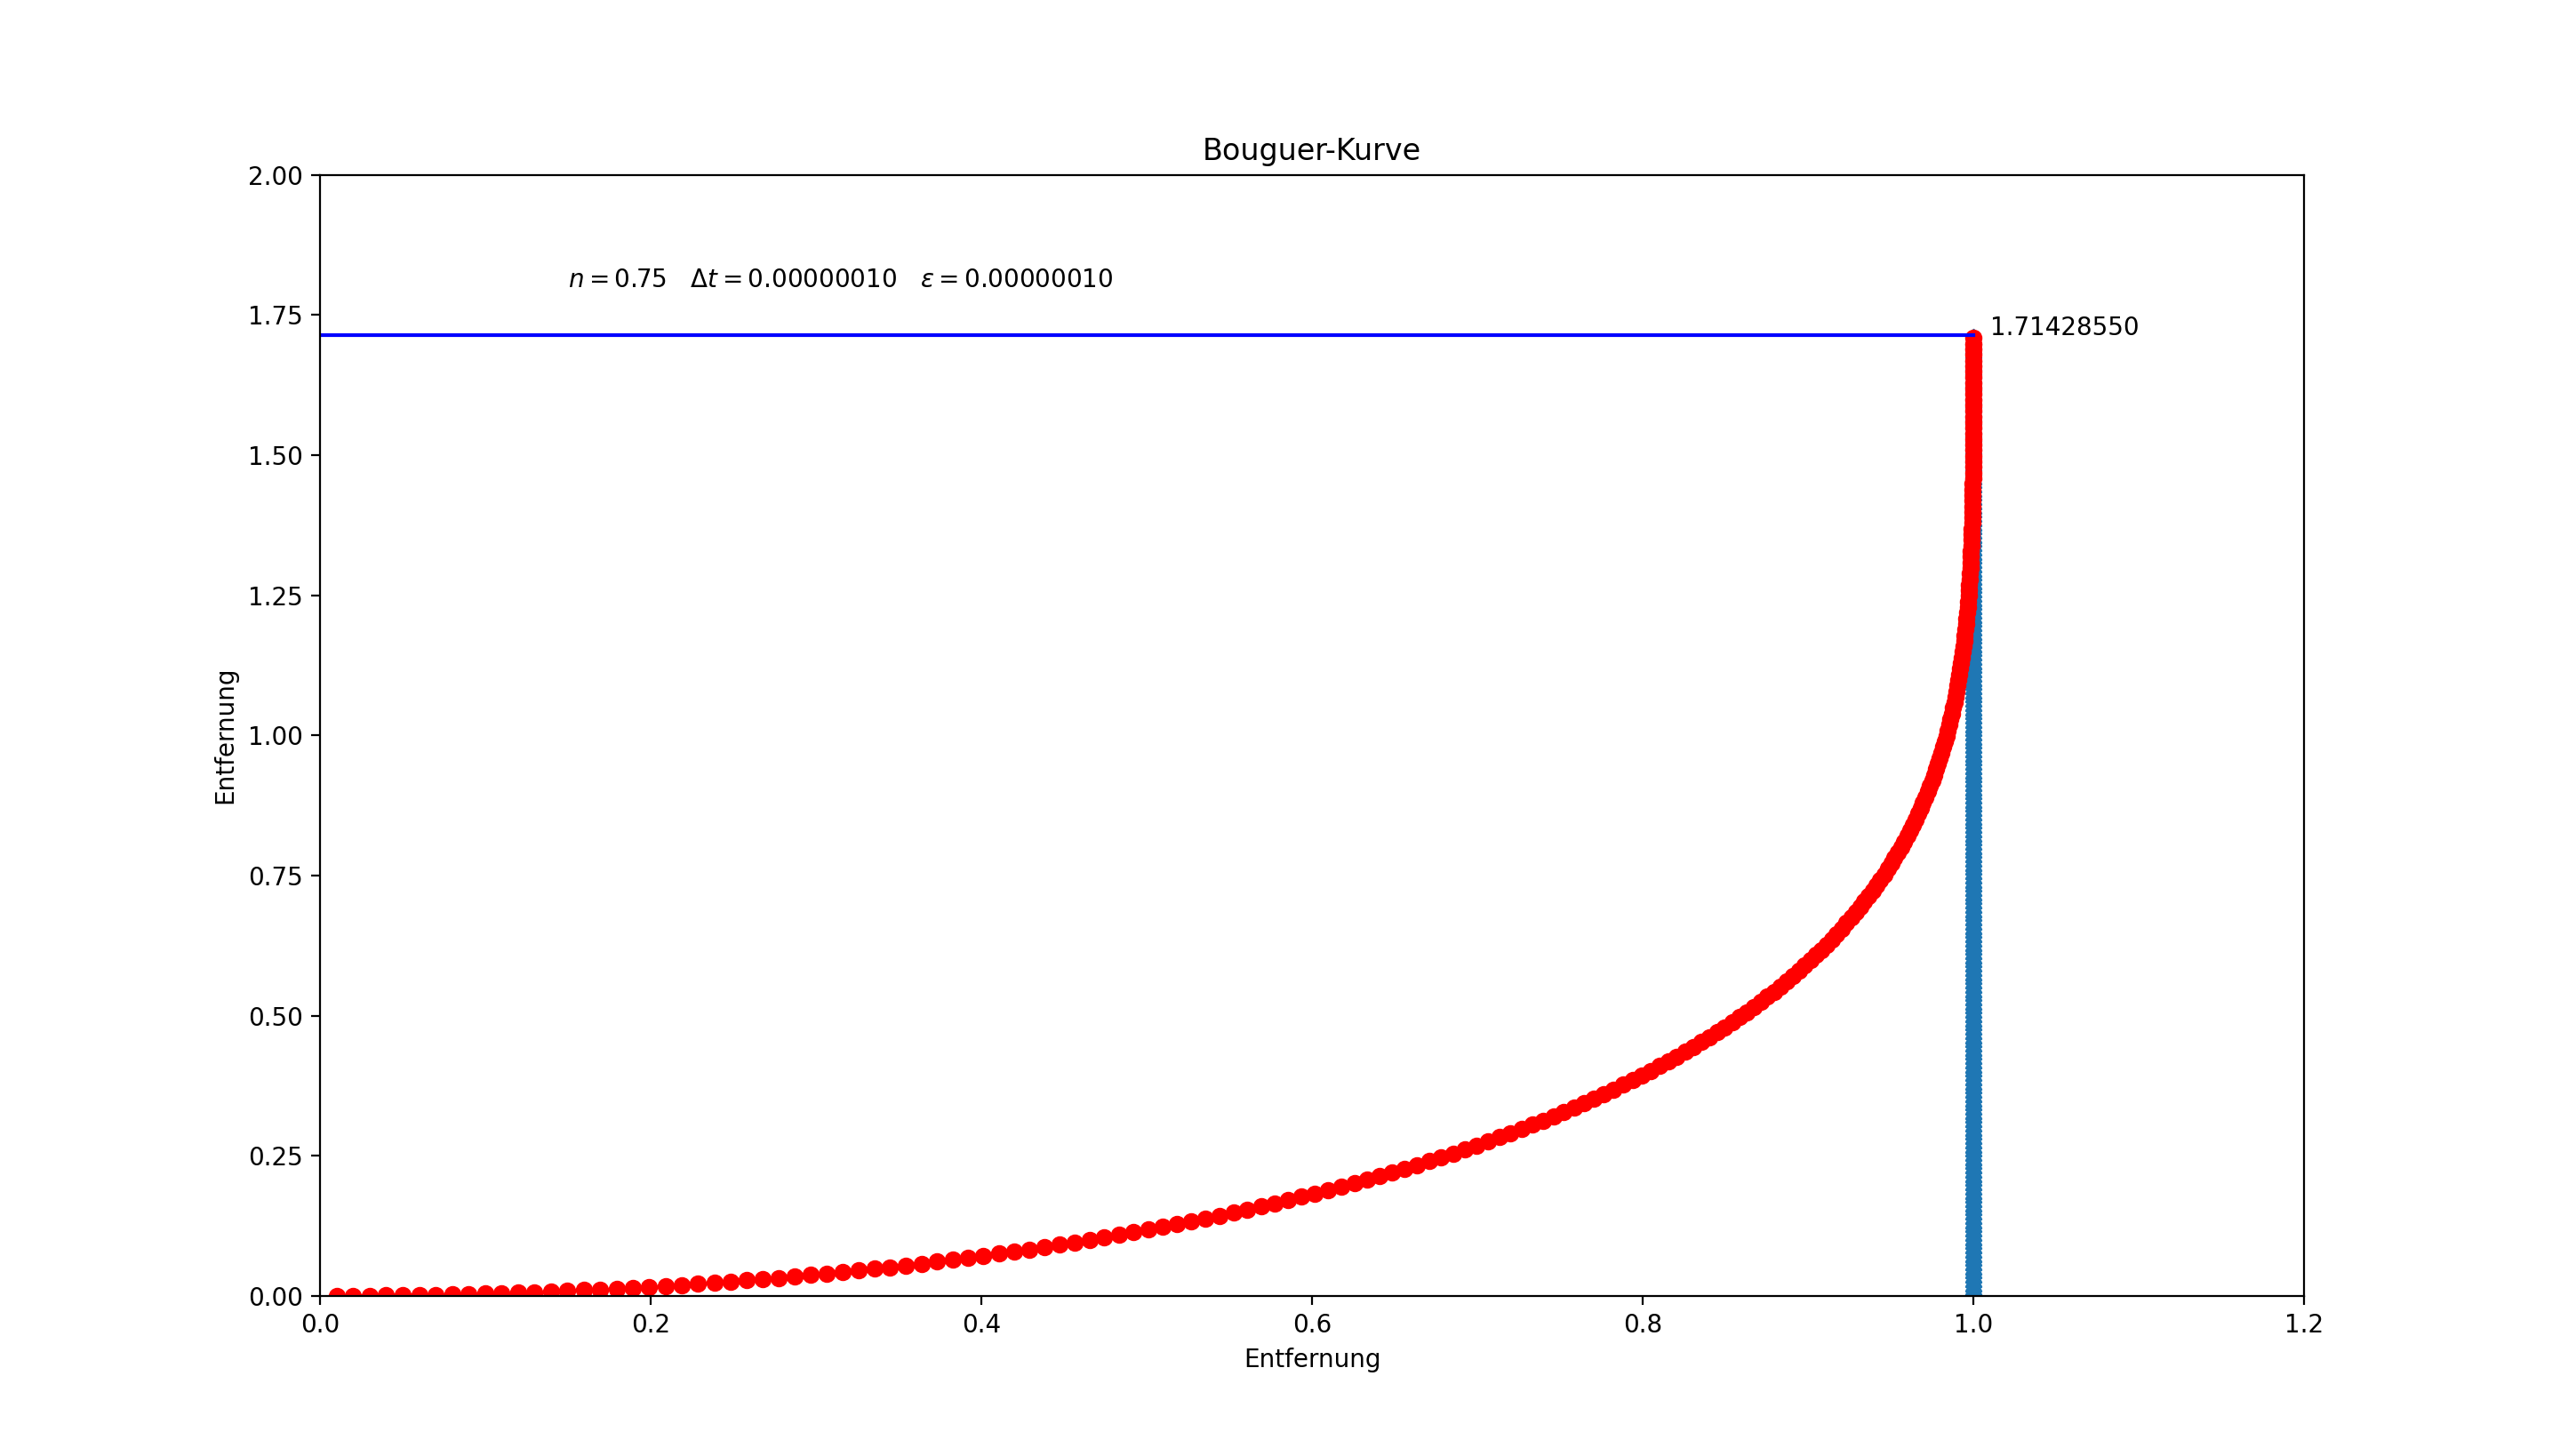
\includegraphics[width=1.02\textwidth]{Aufgabe03.png}

Grafische Ausgabe von \texttt{Aufgabe03Simple.py}
\end{center}
\begin{center}
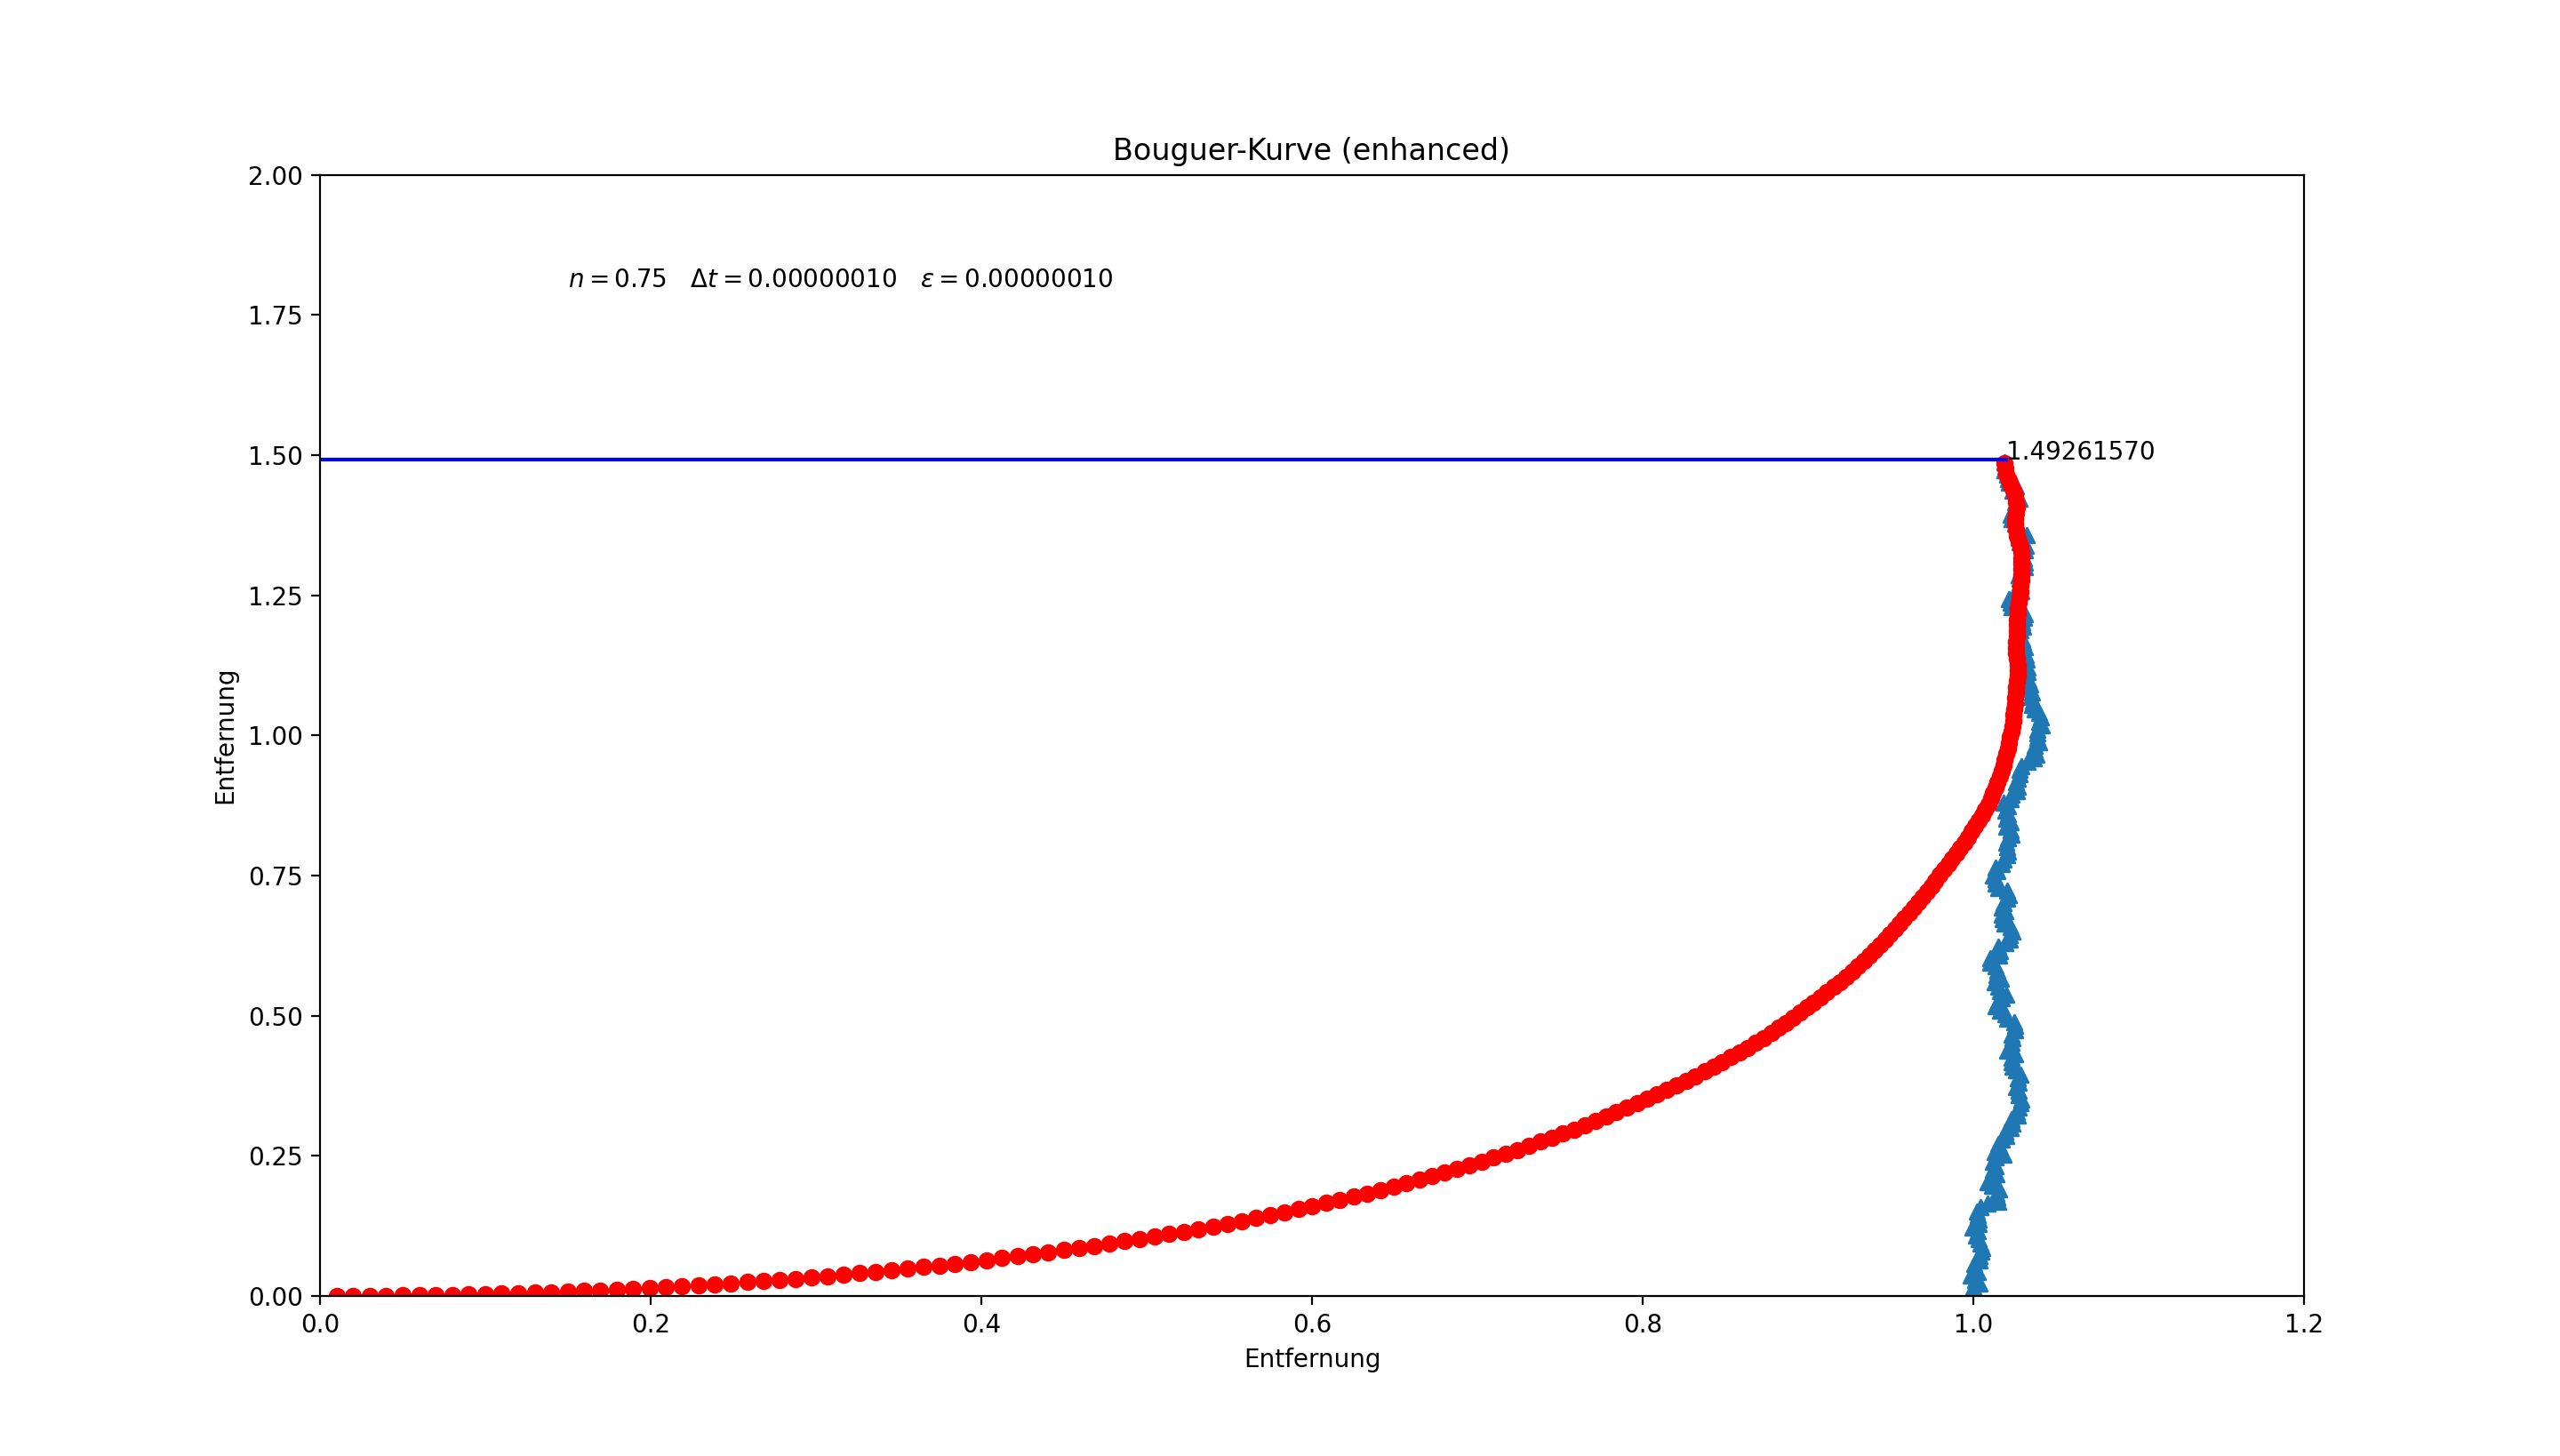
\includegraphics[width=1.02\textwidth]{Aufgabe03Enhanced.png}

Grafische Ausgabe von \texttt{Aufgabe03Enhanced.py}
\end{center}
\newpage
\mylisting[label=musterloesung1]{Musterlösung}{pirate.c}{c}
\mylisting[label=musterloesung2]{Musterlösung}{Aufgabe03Simple.py}{python}
\mylisting[label=musterloesung3]{Musterlösung}{Aufgabe03.py}{python}
\mylisting[label=musterloesung4]{Musterlösung}{Aufgabe03Enhanced.py}{python}

\fi
\end{document}